\chapter{Construção}
\label{cha:Construção}

Com a modelagem da interface e dos dados, foi possível desenvolver o algoritmo e o sistema. O desenvolvimento foi dividido em partes: definição das tecnologias utilizadas, método de coleta dos dados, definição e implementação do algoritmo, e implementação do sistema (interface, API e microserviços). Cada uma das partes está explicada e descrita nas seções a seguir.

\section{Tecnologias utilizadas}
\label{sec:Tecnologias utilizadas}

Para o armazenamento e consulta dos dados, foi utilizado o banco de dados relacional PostgreSQL \cite{site-postgresql}. O PostgreSQL foi escolhido por ser robusto e eficiente, mas fácil e rápido de configurar. 

\begin{figure}[h!]
    \begin{center}
    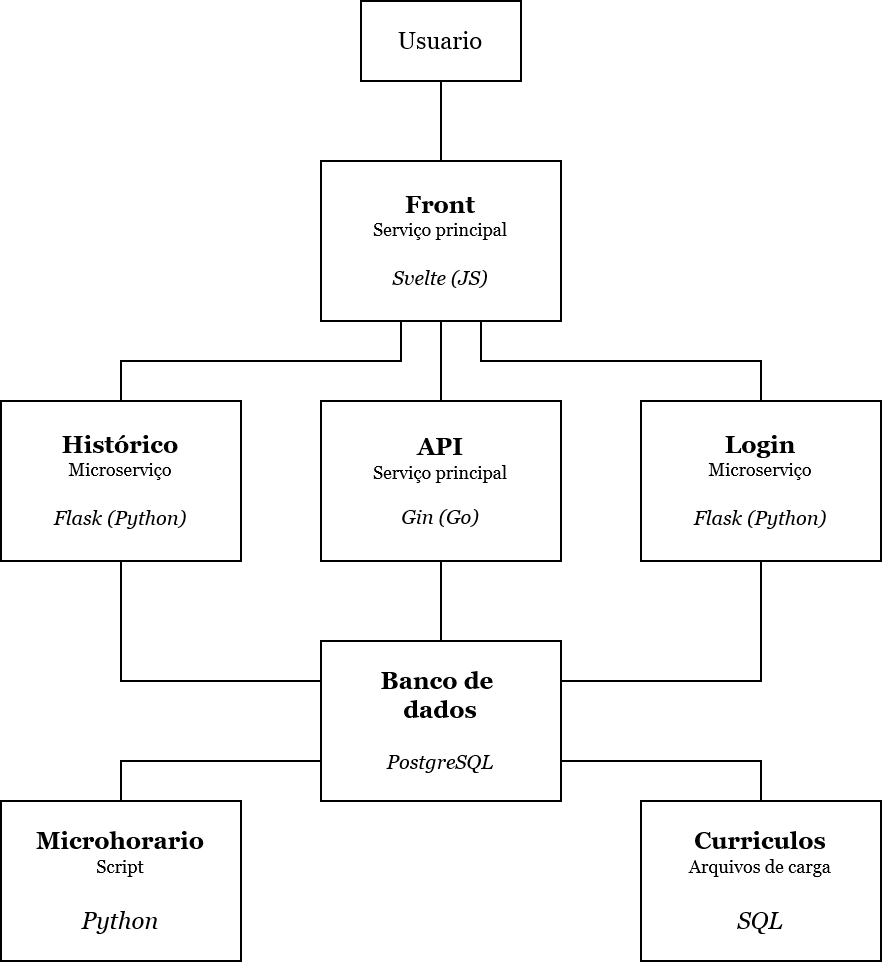
\includegraphics[width=300pt]{figuras/diagrama-arquitetura.png}
    \caption{Diagrama da arquitetura do sistema}
    \label{fig:diagrama-arquitetura}
    \end{center}
\end{figure}

A figura \ref{fig:diagrama-arquitetura} exibe um diagrama da arquitetura do sistema. O sistema foi separado em interface e API (\textit{Application programming interface}, ou interface de programação da aplicação). A coleta dos dados provenientes do Microhorario, a autenticação com o Sistema Acadêmico Universitário e carga/processamento dos históricos foi desenvolvida em serviços menores uma única funcionalidade respectivamente (microserviços). 

As tecnologias utilizadas na API, nos microserviços e na interface estão descritas respectivamente nas seções \ref{sec:Implementação da API}, \ref{sec:Implementação dos microserviços} e \ref{sec:Implementação da interface}.

\section{Coleta de dados}
\label{sec:Coleta de dados}

O modelo lógico representado na figura \ref{fig:modelo-logico} define a construção de catorze tabelas no banco de dados. O trecho de código \ref{cod:sql-create} contém o modelo físico do banco de dados, ou seja o código SQL que define a criação das tabelas.

\lstinputlisting[label=cod:sql-create,title={create.sql},caption={Modelo físico},language=SQL]{codigo/10-create.sql}

No modelo físico, é possível observar que as avaliações, históricos e currículos devem ser sempre associados às disciplinas, através das chaves estrangeiras. Portanto, as disciplinas não podem ser excluídas, mesmo que elas possam não estar sendo oferecidas no semestre atual. Para diferenciar uma disciplina que está sendo oferecida de uma disciplina que não está disponível, basta verificar se ela existe na tabela \verb|turmas|.

No modelo físico, existe a criação de uma tabela \verb|modificacao|, que não estava prevista no modelo lógico. Essa tabela não contém dados relacionais, mas apenas três valores armazenados em uma só linha da tabela. Esses valores representam as datas de coleta das informações das disciplinas e turmas, e se os dados estão em modo de \verb|fallback|, que será explicado na seção \ref{sec:Microhorário no fim do período}.

Além dos dados gerados pela interação do usuário, o sistema precisa de dados provenientes da faculdade, como as disciplinas, turmas, professores e currículos. Esses dados são coletados ocasionalmente, exceto os currículos, que foram manualmente construídos a partir de informações disponíveis nas plataformas da universidade. Como o algoritmo e o sistema foram planejado para alunos do Departamento de Informática, a quantidade de currículos a ser inserida é pequena. No total, foram inseridos seis currículos: três de engenharia de computação (Currículos 2023, 2018.0 e 2018.1) e três de ciência de computação, disponíveis nas respectivas páginas
\footnote{\url{https://www.puc-rio.br/ensinopesq/ccg/eng_computacao.html}}
\footnote{\url{https://www.puc-rio.br/ensinopesq/ccg/ciencia_computacao.html}}
dos cursos.

Os dados de cada currículo foram transformados manualmente em um arquivo no formato SQL que insere o código do currículo e constrói uma \verb|PROCEDURE|, um procedimento responsável por inserir as disciplinas referentes ao currículo. As disciplinas estão dentro de uma \verb|procedure| pois esta deve ser executada toda vez que uma disciplina nova possa ter sido inserida no banco. Isso é necessário pois a \verb|procedure| armazena somente o código de disciplinas que existem no banco, devido a restrição de chave estrangeira da tabela. Portanto, cada vez que uma disciplina nova é inserida, essa operação precisa ser refeita. O trecho de código \ref{cod:sql-curriculo} contém um exemplo de um dos seis arquivos criados, um para cada currículo.

\lstinputlisting[label=cod:sql-curriculo,title={curriculo-cie-18-0.sql},caption={Exemplo do arquivo de carga de currículos},language=SQL]{codigo/10-curriculos.sql}

Os dados provenientes das disciplinas e turmas são coletados diretamente através do microhorário. Foi criada uma biblioteca Python que permite baixar todos as informações disponíveis no microhorário, e opcionalmente coletar as ementas e pré-requisitos que estão disponíveis em página. A biblioteca baixa os dados das disciplinas e turmas em menos de três segundos, mas pode executar por até 30 minutos para baixar as ementas e pré-requisitos que estão em outro serviço da universidade. Portanto, foi criado um módulo, chamado \verb|microhorario|, que permite atualizar o banco com as informações básicas das disciplinas e turmas, mas que pode ser alterado para atualizar também as ementas e pré-requisitos. Esse módulo foi configurado de forma a ser executado na sua forma mais simples (somente atualiza os dados referentes às turmas) uma vez a cada hora, e executado na forma completa (coleta inclusive as ementas e pré-requisitos) uma vez por dia.

\subsection{Microhorário no fim do período}
\label{sec:Microhorário no fim do período}

No final de cada período, devido a preparação das disciplinas e turmas para o próximo semestre, o microhorário não disponibiliza dados como quantidade de vagas e quantidade de créditos. Por isso, foi necessário que o sistema e o algoritmo acomodasse essas necessidades temporárias. Nesse caso, a variável de \verb|fallback|, presente na tabela de \verb|modificacao| estará no seu valor verdadeiro. Se o microhorário estiver disponível, essa variável está com seu valor falso.

\subsection{Disciplinas optativas}
\label{sec:Disciplinas optativas}

Os currículos contém grupos de disciplinas optativas. Cada grupo de disciplinas optativas possuem várias disciplinas, e o aluno deve cursar pelo menos uma delas para que seja considerado o grupo como cursado. Por exemplo, o currículo de 19.0 de Engenharia de Computação determina o grupo de optativa \verb|INF0303|, com as disciplinas \verb|ENG1456 - INTELIGENCIA COMPUT APLICADA| e \verb|INF1771 - INTELIGENCIA ARTIFICIAL|, e o aluno deve necessariamente cursar uma das duas. Essa categoria de disciplinas não foi percebida durante todo o processo de entrevistas, levantamento de requisitos e modelagem do banco. Para implementar essa categoria de forma eficaz, seria necessária uma reestruturação das tabelas do banco de dados, e diversas alterações complexas nos módulos de coleta de dados do microhorário e dos outros serviços, inclusive alterações na biblioteca de consulta ao microhorário citada acima. Portanto, optou-se por não implementar as disciplinas optativas. Em vez disso, as disciplinas relacionadas ao grupo de optativas não são atreladas ao currículo, sendo consideradas eletivas.

\subsection{Co-requisitos}
\label{sec:Co-requisitos}
Durante o desenvolvimento de coleta de dados da ementa, foi observado que algumas disciplinas possuem co-requisitos. Co-requisitos são disciplinas que precisam ser cursadas no mesmo período, conforme a imagem \ref{fig:corequisito}. Como esse atributo foi descoberto no momento que o desenvolvimento já estava em andamento, optou-se por não implementar essa funcionalidade. Em vez disso, nenhuma disciplina possui co-requisitos.

\begin{figure}[ht]
    \begin{center}
    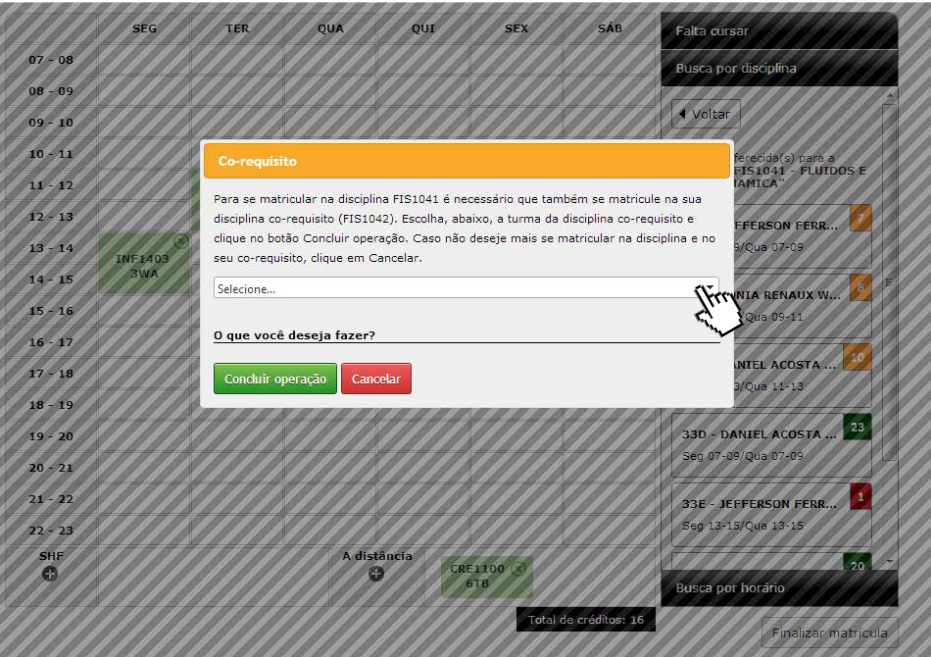
\includegraphics[width=350pt]{figuras/corequisitos.png}
    \caption{Seleção de uma disciplina com co-requisitos durante o processo de matrícula}
    \label{fig:corequisito}
    \end{center}
\end{figure}

\subsection{Quantidade de créditos}
Durante a fase de entrevistas, foi solicitado a média de créditos das grades horários dos entrevistados. O objetivo era possivelmente alimentar o algoritmo de recomendação com essa média para, por exemplo, recomendar disciplinas com menos créditos caso o aluno estivesse chegando nessa média. Porém, não foi possível criar um bom modelo matemático utilizando essa informação, por isso ela foi descartada na implementação atual.


\section{Definição e implementação do algoritmo}
\label{sec:Definição e implementação do algoritmo}

O algoritmo busca satisfazer as necessidades apresentadas na tabela \ref{tab:entrevista-criterios-peso}. As entrevistas indicaram a importância de cinco categorias (Conteúdo, Professor, Avaliação, Horário e Opinião). Por isso, o algoritmo foi dividido nessas cinco categorias.

O algoritmo se baseia num valor $V[d,u]$ atribuído a cada disciplina, que indica a relevância da disciplina $d$ para o usuário $u$. O valor $V[d,u] \in [0, 1]$,
sendo 1 o maior grau de relevância da disciplina, e 0 o menor. O cálculo de $V$ é uma média ponderada, conforme a equação \ref{equ:algoritmo-valor}.

\begin{multline}
\label{equ:algoritmo-valor}
    V[d,u] = \\
        P_cV_c[d,u] + P_pV_p[d] + P_oV_o[d] + P_hV_h[d,u] + P_aV_a[d]
\end{multline}

Em que $d$ é uma disciplina, $u$ é um usuário, $V_x$ é o valor de uma das cinco categorias para a disciplina $d$ e o usuário $u$, e $P_x$ é o peso de uma das cinco categorias. Por exemplo, $P_cV_c[d,u]$ se refere ao cálculo do conteúdo, $P_pV_p[d]$ se refere ao cálculo do professor, e assim por diante.

%% valor V_c

O valor $V_c[d,u]$ indica o quão relevante é a disciplina para o usuário de acordo com o seu conteúdo. Para isso, o valor é calculado de acordo com o histórico de outros alunos e com o currículo do aluno, conforme a equação \ref{equ:algoritmo-conteudo}.

\begin{equation}
    V_c[d,u] = 
    \begin{dcases}
        \hfil 1.0 & \text{caso} \: d \in Historico[u] \\ 
        \frac{|\, A_{cursou}[d,u] \,|}{|\,  A_{curriculo}[u] \,|}   & \text{caso} \: A_{curriculo}[u] > 0 \\
        0 & \text{caso contrário}
    \end{dcases} \\[20pt]
    \label{equ:algoritmo-conteudo}
\end{equation}

Em que:

\begin{align*}
    & A_{curriculo}[u] = \forall a \in Alunos \,|\, Curriculo[a] = Curriculo[u] \\
    & A_{cursou}[d,u] = \forall a \in A_{curriculo}[u] \,|\, d \in Cursadas[a] \\
\end{align*}

Em que $d$ é uma disciplina, $u$ é um usuário, $Alunos$ é o conjunto de todos os usuários cadastrados no sistema, $Curriculo[u]$ é o currículo do usuário $u$, e $Cursadas[u]$ é o conjunto de disciplinas que o aluno $u$ cursou. Em resumo, o valor $V_c[d,u]$ é o valor máximo caso a disciplina deve ser cursada pelo usuário, ou sendo uma eletiva é a proporção de alunos do mesmo currículo que fizeram esta disciplina. Essa proporção indica se o conteúdo é relevante para alunos semelhantes ao usuário.

%% Valor V_p

O valor $V_p[d]$ indica o quão relevante é a disciplina para o usuário de acordo com o professor. Para isso, o valor é calculado de acordo com as avaliações dos professores das turmas das disciplinas, conforme a equação \ref{equ:algoritmo-professor}.

\begin{equation}
    V_p[d] = \frac{\sum_{p \in P[d]} \displaystyle  \frac{\sum_{a \in Avs[p]} a}{| Avs[p] |}}{| P[d] |} \,/\, 5
    \label{equ:algoritmo-professor}
\end{equation}

Em que $d$ é uma disciplina, $P[d]$ é o conjunto dos professores que lecionam a disciplina $d$, e $Avs[p]$ representa o conjunto das avaliações dos usuários do professor $p$. Em resumo, o valor $V_p[d8]$ é a média das avaliações de todos os professores que estão lecionando a disciplina, com o valor entre $0$ e $1$.

%% Valor V_o

O valor $V_o[d]$ indica o quão relevante é a disciplina para o usuário de acordo com a opinião dos alunos. A equação é semelhante ao cálculo apresentado na equação \ref{equ:algoritmo-professor}. Porém, nesse caso, é levado em conta a média das avaliações das próprias disciplinas, conforme a equação \ref{equ:algoritmo-opiniao}.

\begin{equation}
    V_p[d] = \frac{\sum_{a \in Op[d]} a} {| Op[d] |} \,/\, 5
    \label{equ:algoritmo-opiniao}
\end{equation}

Em que $d$ é uma disciplina, e $Op[d]$ é o conjunto das avaliações dos usuários da disciplina $d$.

%% Valor V_h

O valor $V_h[d,u]$ indica o quão relevante é a disciplina para o aluno de acordo com o horário. Para isso, o valor é calculado de acordo com os horários ocupados na grade do usuário e os horários das disciplinas, conforme a equação \ref{equ:algoritmo-horario}

\begin{equation}
    V_h[d,u] = 
    \begin{dcases}
        \frac{|\, T_{possiveis}[d,u] \,|}{|\,  T[d] \,|}   & \text{caso} \: T[d] > 0 \\
        \hfil 0 & \text{caso contrário}
    \end{dcases} \\[20pt]
    \label{equ:algoritmo-horario}
\end{equation}

Em que $d$ é uma disciplina, $u$ é um usuário, $T_{possiveis}[d,u]$ é o conjunto de turmas da disciplina $d$ que se encaixam na grade do usuário $u$, e $T[d]$ é a quantidade de turmas da disciplina $d$. Em resumo, $V_h[d, u]$ é a porcentagem de turmas da disciplina que se encaixam na grade do usuário.

Por último, o valor $V_a[d]$ indica o quão relevante é a disciplina para o aluno de acordo com os graus (a nota final, considerando as provas do aluno durante o semestre) da disciplina. O cálculo é semelhante às equações \ref{equ:algoritmo-professor} e \ref{equ:algoritmo-opiniao}, conforme a equação \ref{equ:algoritmo-avaliacao}.

\begin{equation}
    V_p[d] = \frac{\sum_{g \in Graus[d]} g} {| Graus[d] |} \,/\, 100 
    \label{equ:algoritmo-avaliacao}
\end{equation}

Em que $d$ é uma disciplina e $Graus[d]$ é o conjunto das notas da disciplina $d$.

Para obter todos os valores dos conjuntos citados nas equações anteriores, foi criada uma consulta SQL que obtém todos os valores de uma só vez. 

O trecho de código \ref{cod:sql-algoritmo} contém a consulta por completo. Antes de executar, são substituidos os valores \verb|@usuario| pelo código do usuário, e o valor \verb|@escolhas| por um trecho de código SQL referente às escolhas de turmas de disciplinas na grade atual do aluno.

\lstinputlisting[label=cod:sql-algoritmo,title={algoritmo.sql},caption={Consulta dos dados para o algoritmo},language=SQL]{codigo/10-algoritmo.sql}

A consulta possui oito consultas auxiliares, sendo sete delas usadas para calcular os valores $V_x$ do algoritmo de recomendação. As explicações das consultas auxiliares estão na lista a seguir:

\begin{itemize}
    \item \verb|rec_c1| Seleciona as disciplinas oferecidas pelo currículo do usuário;
    \item \verb|rec_c2_1| Seleciona a quantidade de alunos do mesmo currículo do usuário por disciplina do currículo do usuário;
    \item \verb|rec_c2_2| Seleciona a quantidade de usuários do mesmo currículo do usuário;
    \item \verb|rec_h| Seleciona, por disciplina, a quantidade de turmas não conflitantes com a grade do usuário e a quantidade total de turmas;
    \item \verb|rec_o| Seleciona as média das avaliações das disciplinas;
    \item \verb|rec_p| Seleciona as médias das avaliações dos professores;
    \item \verb|rec_a| Seleciona as médias dos graus dos alunos por disciplina;
    \item \verb|filtro| Seleciona as disciplinas que o usuário não cursou. 
\end{itemize}

Por fim, os pesos $P_x$ da média ponderada foram baseados na tabela \ref{tab:entrevista-criterios-peso}. Cada peso é a soma dos pesos dos critérios, de acordo com as equações a seguir.

\begin{align}
    & P_c = \frac{41}{41 + 19 + 8 + 28 + 21} \\[10pt]
    & P_p = \frac{28}{41 + 19 + 8 + 28 + 21} \\[10pt]
    & P_o = \frac{ 8}{41 + 19 + 8 + 28 + 21} \\[10pt]
    & P_h = \frac{19}{41 + 19 + 8 + 28 + 21} \\[10pt]
    & P_a = \frac{21}{41 + 19 + 8 + 28 + 21}
\end{align}

\section{Implementação da API}
\label{sec:Implementação da API}

A API é responsável por servir disponibilizar à interface os dados de forma organizada e eficaz. Foi estudada a implementação da API em quatro possíveis frameworks em três diferentes linguagens:
\textit{Django} \cite{site-django}, \textit{Flask} \cite{site-flask}, \textit{Gin} \cite{site-gin} e \textit{Rocket} \cite{site-rocket}. Cada um dos frameworks possui suas vantagens e desvantagens.

O framework \textit{Django} é um \textit{Web Framework} completo, que possui múltiplas funcionalidades pré-configuradas, possui uma interface de comunicação com banco de dados bem robusta. O framework \textit{Flask} por sua vez não possui muitas funcionalidades embutidas, e depende da instalação de pacotes externos para ampliar suas funcionalidades. Ambos os frameworks são desenvolvidos na linguagem Python, o que torna o desenvolvimento mais fácil, mas reduz performance do funcionamento, por ser uma linguagem interpretada.

O framework \textit{Rocket} é desenvolvido na linguagem Rust \cite{site-rust}, conhecida por ser rápida e segura, por possuir um abordagem de manipulação de memória diferente de outras linguagens. Porém, Rust possui uma alta curva de aprendizado, dificultando o desenvolvimento do código.

Por fim, o framework \textit{Gin} é desenvolvido na linguagem Go \cite{site-go}, conhecida por bem eficiente, útil para o desenvolvimento de APIs pelo sua capacidade de multiprocessamento, e fácil de usar. Por isso, esse framework foi escolhido para a API do sistema.

A API disponibiliza a documentação completa de todas as suas rotas, com as respectivas entradas e saídas, conforme a figura \ref{fig:api}.

\begin{figure}[ht]
    \begin{center}
    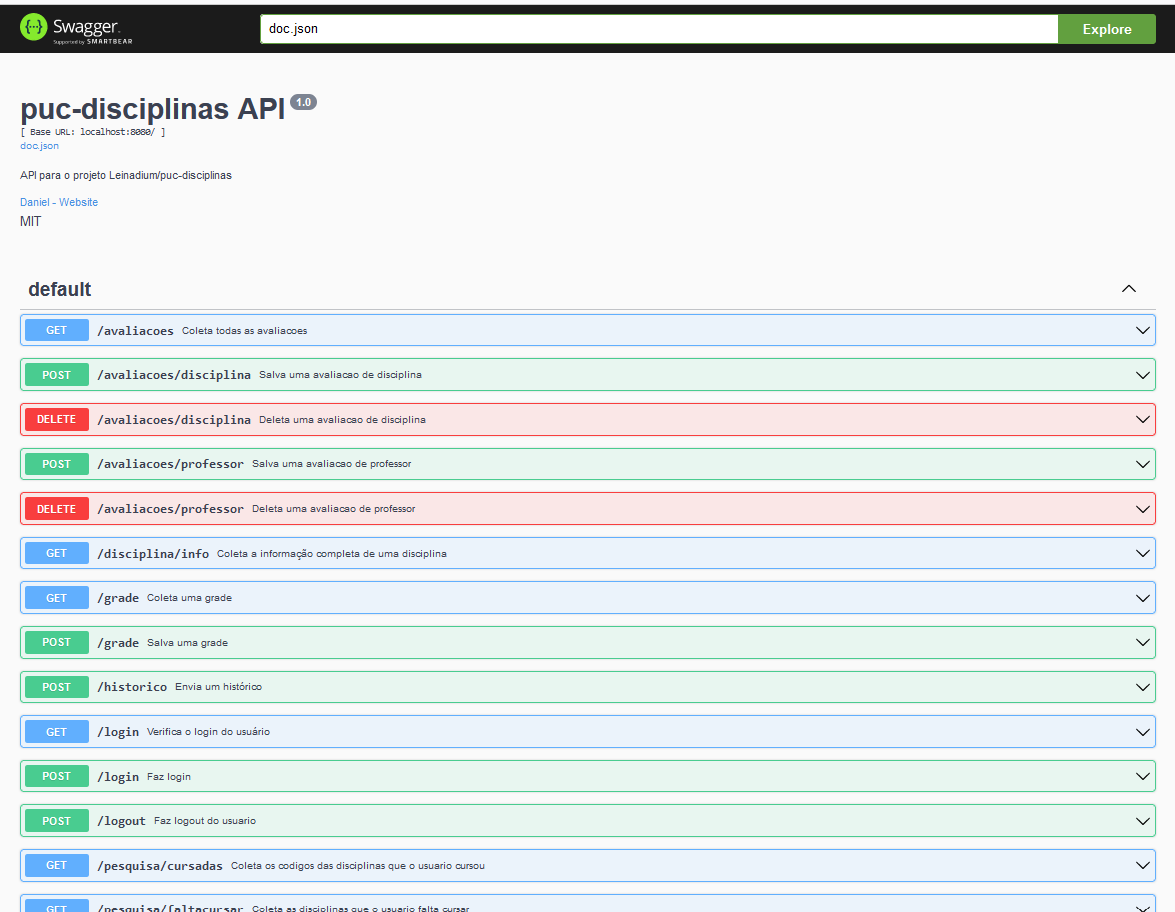
\includegraphics[width=360pt]{figuras/api.png}
    \caption{Documentação da API}
    \label{fig:api}
    \end{center}
\end{figure}

\section{Implementação dos microserviços}
\label{sec:Implementação dos microserviços}

Os serviços de autenticação, e de carga e processamento dos históricos dos alunos são processos separados da API. Ambos foram desenvolvidos na linguagem Python, por sua facilidade de processamento dos dados, e por não haver a necessidade uma performance ótima. Esses utilizam o framework Flask para disponibilizar os serviços, por serem serviços bem simples.

O serviço de autenticação se comunica com o Sistema Acadêmico Universitário (SAU). Existe uma API para autenticação dos alunos da universidade, mas é restrita para os serviços interno da mesma. Por isso, o serviço de autenticação implementado simula um aluno autenticando-se no portal \footnote{Disponível em: \url{https://www.puc-rio.br/ensinopesq/academicas/}, Sistemas Acadêmicos - SAU} do SAU, e verifica se a autenticação foi efetuada com sucesso.

O serviço de carga dos históricos precisa receber como entrada a página do histórico do usuário. É possível coletar o histórico de forma automática, acessando o portal do SAU também simulando um usuário. Porém, como essa interação com o SAU não seria transparente com o usuário, sendo executado de forma oculta, não foi considerada a melhor opção. Por isso, optou-se pelo usuário salvando uma cópia da página do seu histórico, e submetendo-o através da interface, que se comunica com o serviço de carga e processamento dos históricos. 

\section{Implementação da interface}
\label{sec:Implementação da interface}

A interface foi implementada utilizando o framework \textit{Svelte}, que permite desenvolver páginas interativas baseadas em componentes. A programação é feita utilizando um misto de Javascript e HTML, que é compilada em pacotes Javascript pequenos que são interpretados pelo navegador de internet. 

Como foi necessário desenvolver pelo menos três páginas diferentes, conforme o wireframe do capítulo \ref{cha:Wireframe}, foi utilizado o framework \textit{SvelteKit} \cite{site-sveltekit}. Este permite disponibilizar páginas desenvolvidas em Svelte em diferentes rotas, além de outras possibilidades, como SSR (\textit{Server-Side Rendering}, ou renderização no servidor), que permite reduzir o esforço do navegador do usuário ao construir inicialmente a página no servidor. 

A seguir estão algumas imagens da interface implementada do sistema. A figura \ref{fig:tela-inicial-impl} mostra a tela inicial, com um menu de seleção para a página de grade e de avaliações. As figuras \ref{fig:tela-grade-impl} e \ref{fig:detalhe-turmas-impl} exibem a interface de criação de grade horária. 
Na figura \ref{fig:tela-grade-impl} é possível observar a mensagem de aviso, caso os dados completos do microhorário estejam indisponíveis.

\begin{figure}[h]
    \begin{center}
    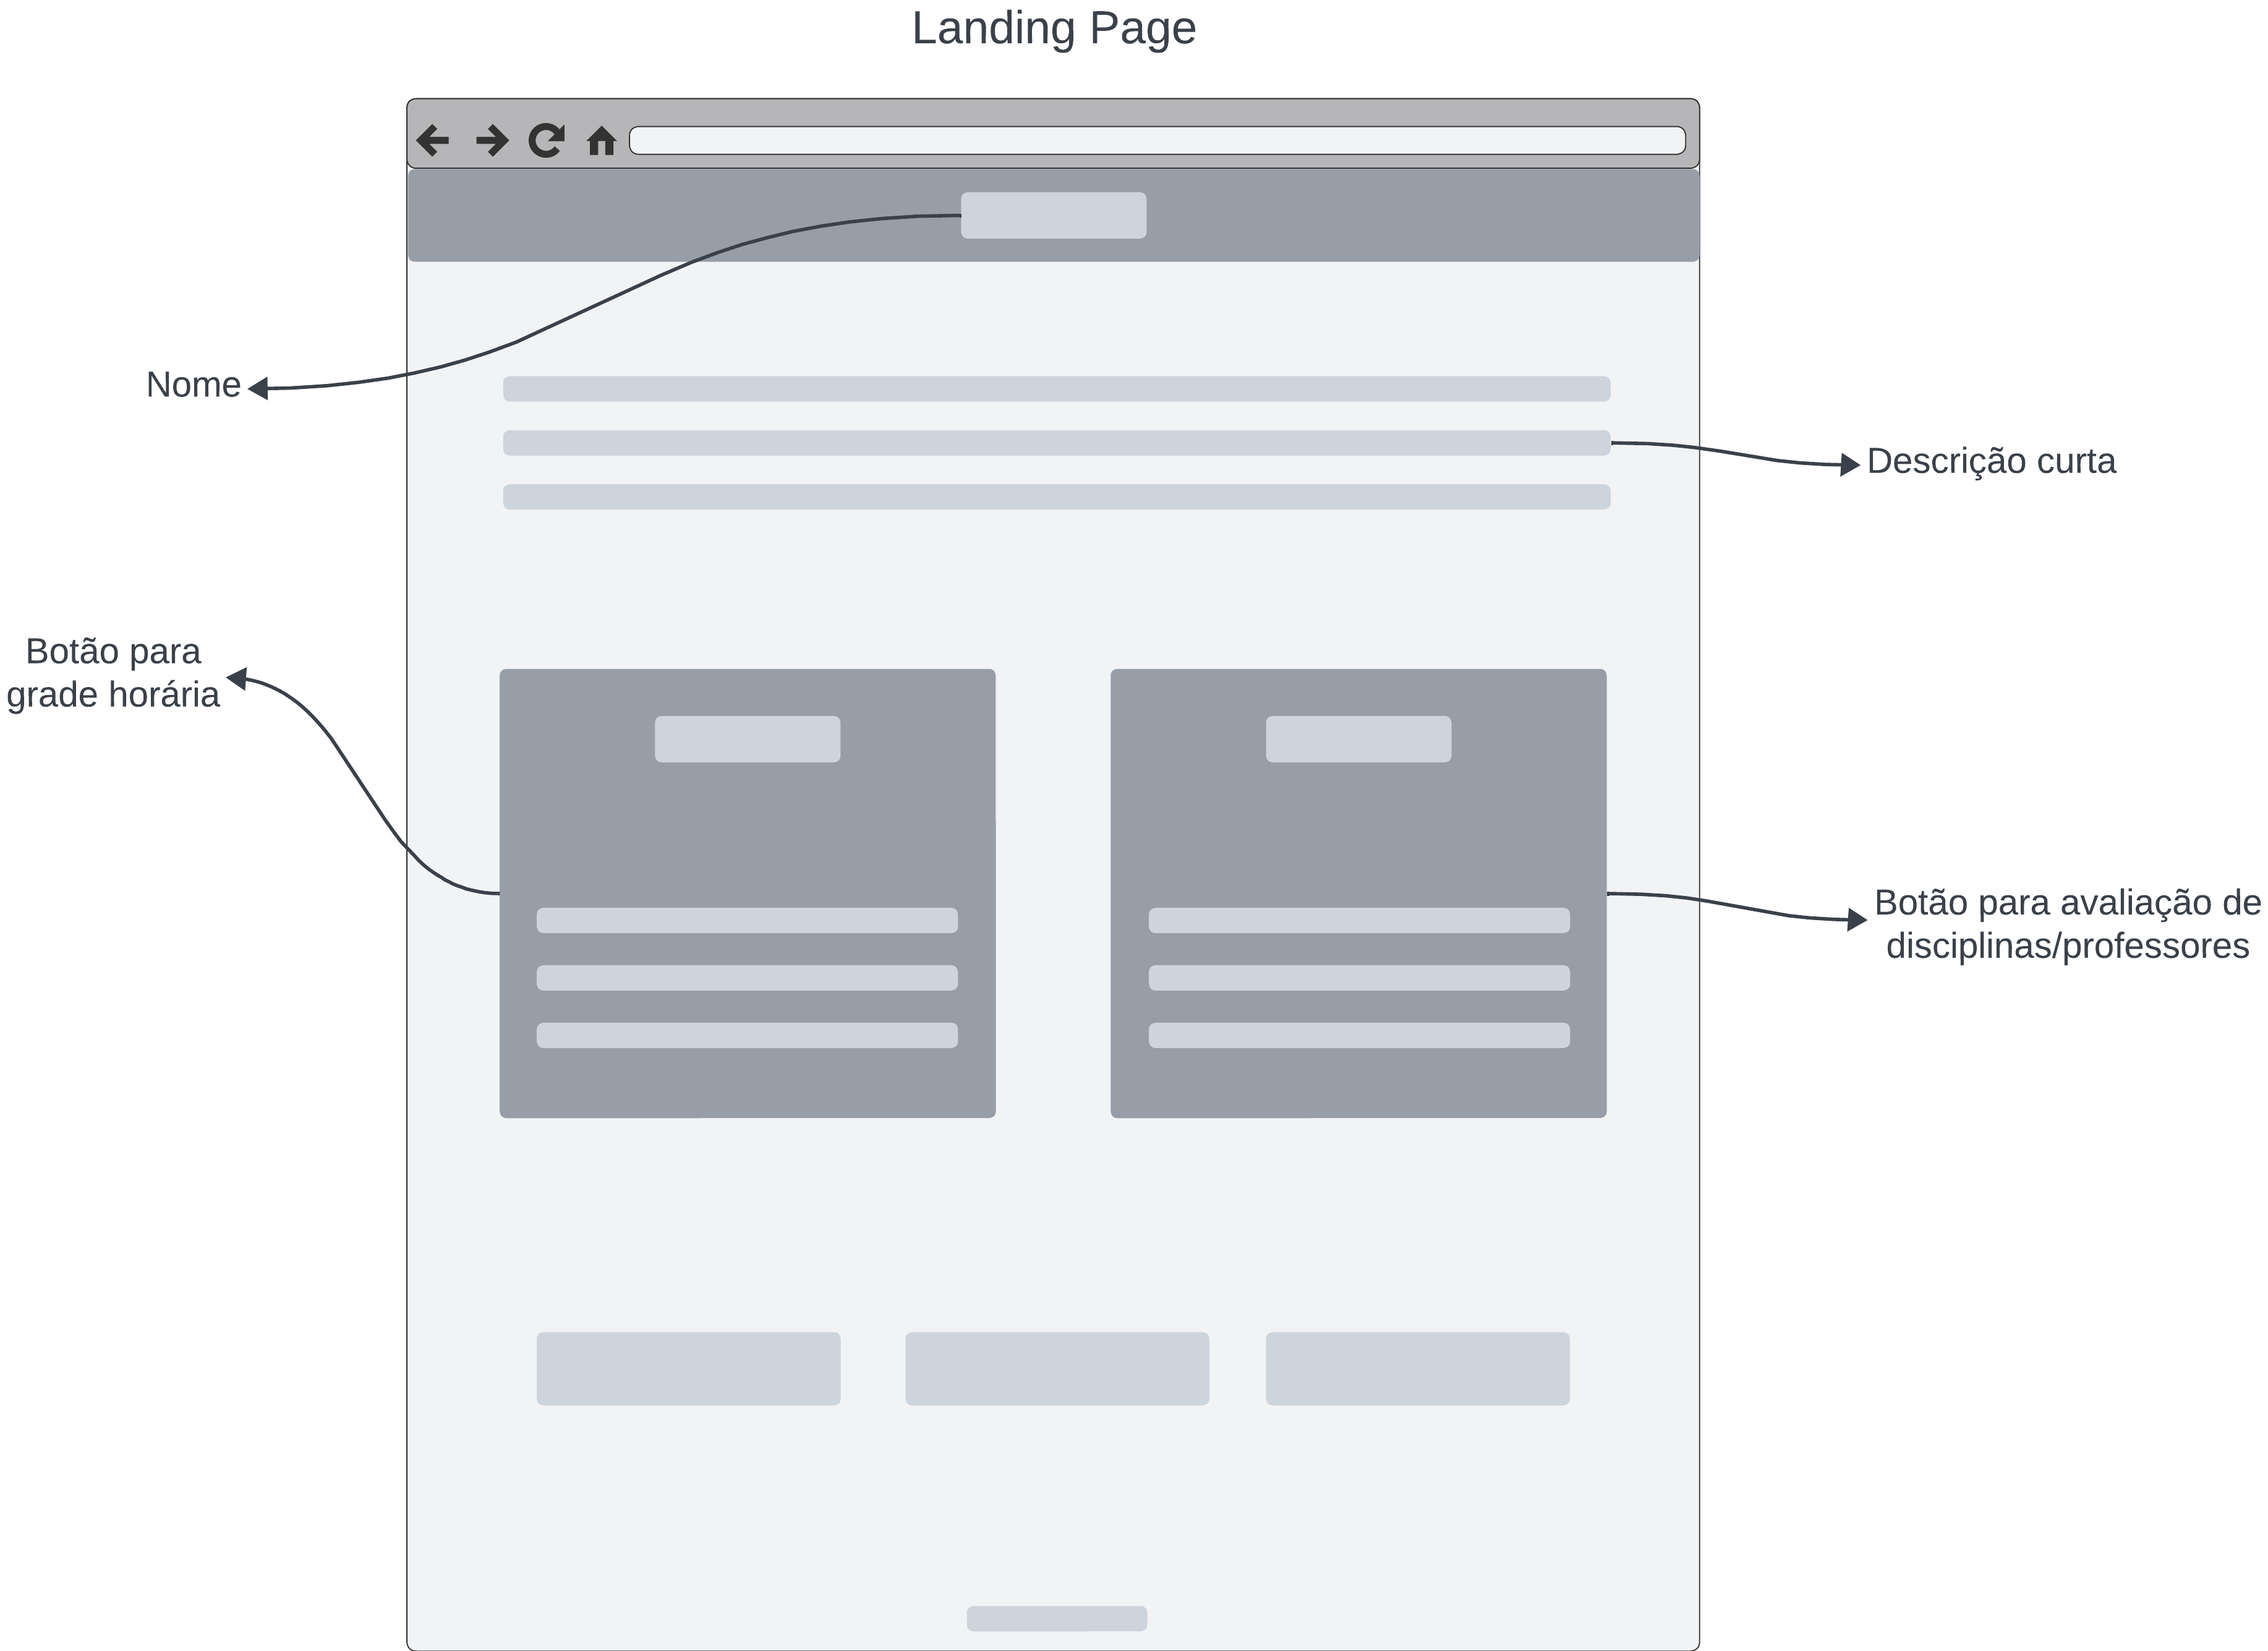
\includegraphics[width=360pt]{figuras/tela-inicial.png}
    \caption{Implementação da tela inicial da interface}
    \label{fig:tela-inicial-impl}
    \end{center}
\end{figure}

\begin{figure}[h]
    \begin{center}
    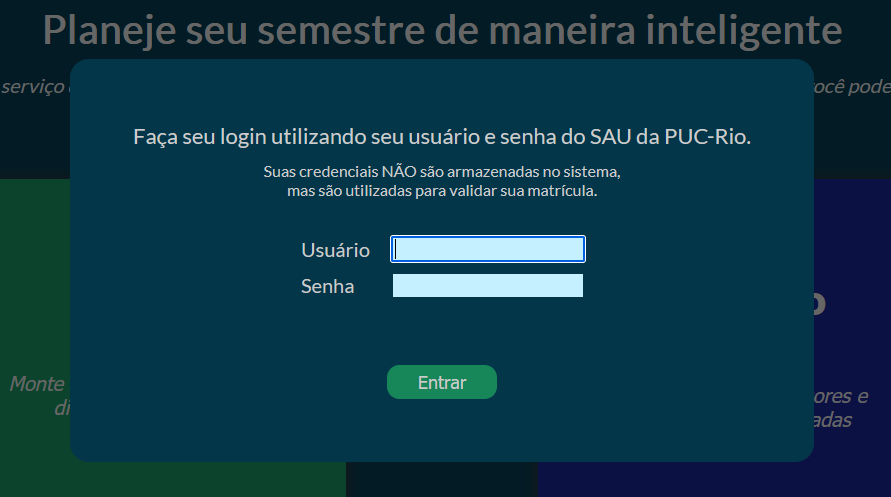
\includegraphics[width=360pt]{figuras/autenticacao-usuario.png}
    \caption{Implementação da tela de autenticação do usuário}
    \label{fig:tela-autenticacao-impl}
    \end{center}
\end{figure}

\begin{figure}[h]
    \begin{center}
    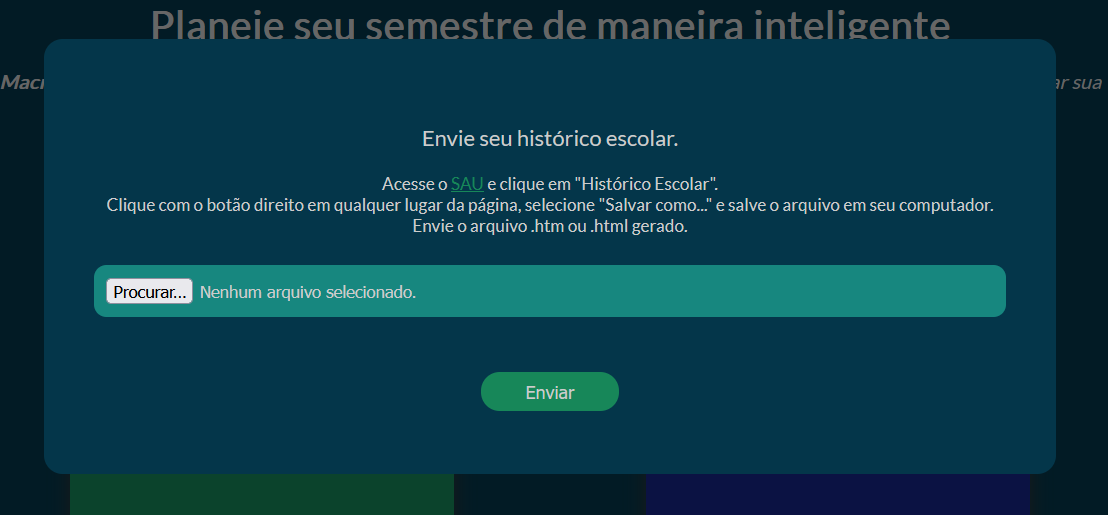
\includegraphics[width=360pt]{figuras/cadastro-historico.png}
    \caption{Implementação da tela de cadastro de histórico}
    \label{fig:tela-historico-impl}
    \end{center}
\end{figure}

\begin{figure}[h]
    \begin{center}
    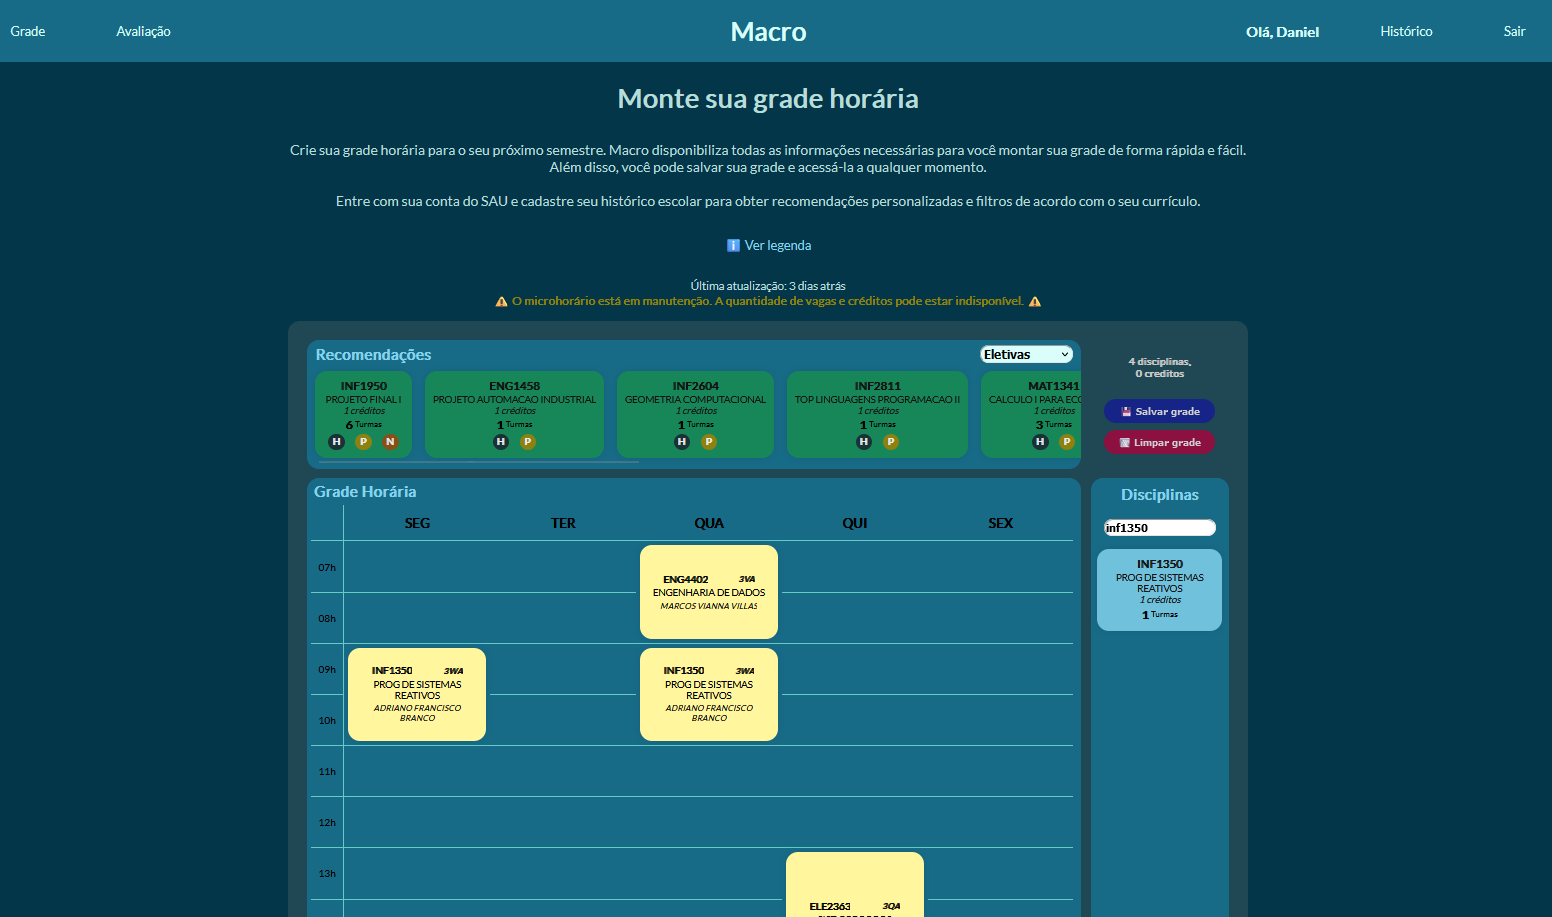
\includegraphics[width=360pt]{figuras/tela-grade.png}
    \caption{Implementação da tela de criação de grade da interface}
    \label{fig:tela-grade-impl}
    \end{center}
\end{figure}

\begin{figure}[h]
    \begin{center}
    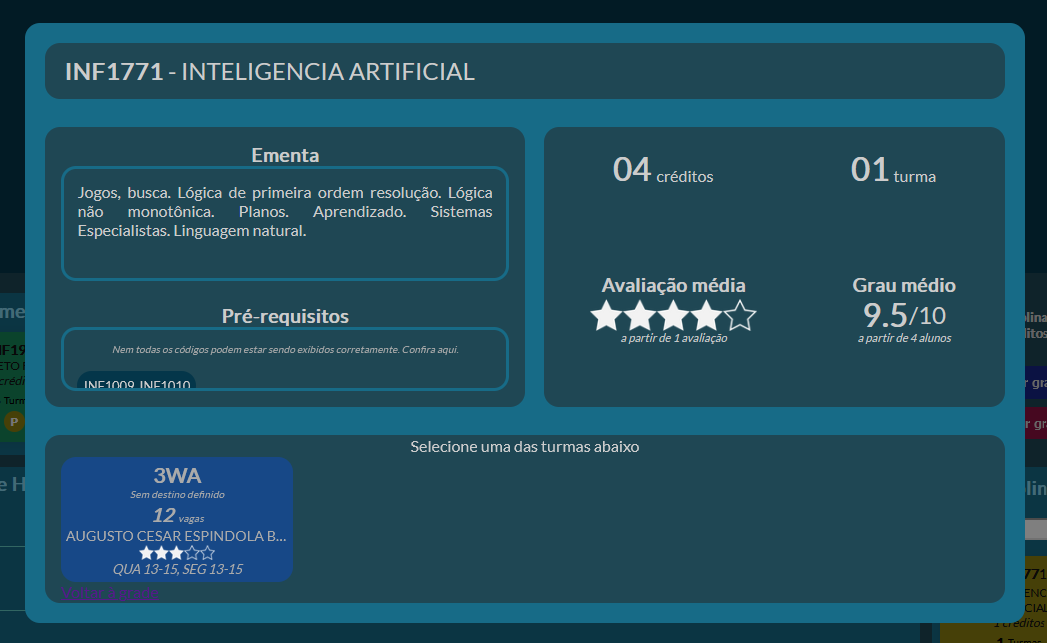
\includegraphics[width=360pt]{figuras/detalhe-turma.png}
    \caption{Detalhes de uma disciplina na interface, exibido ao selecionar uma disciplina}
    \label{fig:detalhe-turmas-impl}
    \end{center}
\end{figure}

\begin{figure}[h]
    \begin{center}
    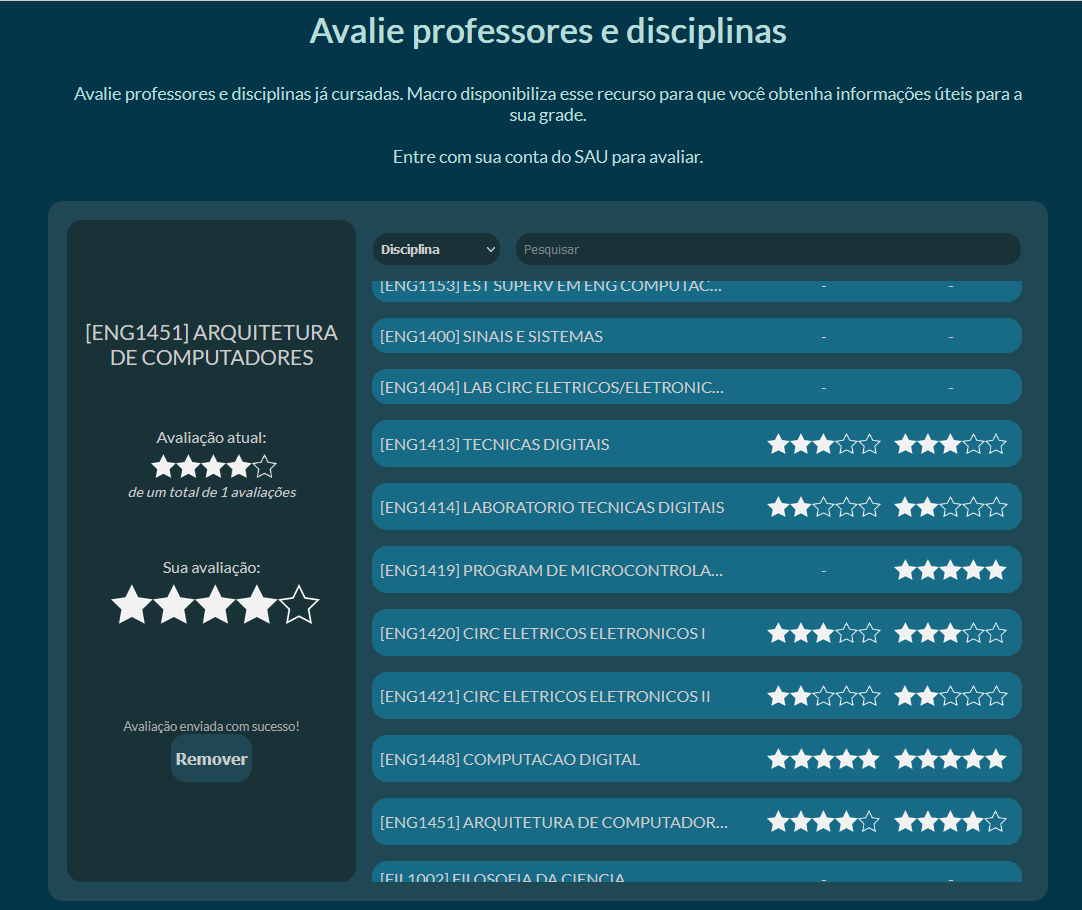
\includegraphics[width=360pt]{figuras/tela-avaliacoes.png}
    \caption{Implementação da tela de avaliação da interface}
    \label{fig:tela-avaliacao-impl}
    \end{center}
\end{figure}

As disciplinas recomendadas podem possuir informações extras. A figura \ref{fig:legenda-interface} mostra uma legenda disponível no sistema explicando as informações exibidas. A figura explica que uma disciplina pode estar sendo recomendada devido a 5 categorias, que estão associadas aos pesos explicados na seção \ref{sec:Definição e implementação do algoritmo}.

\begin{figure}[ht]
    \begin{center}
    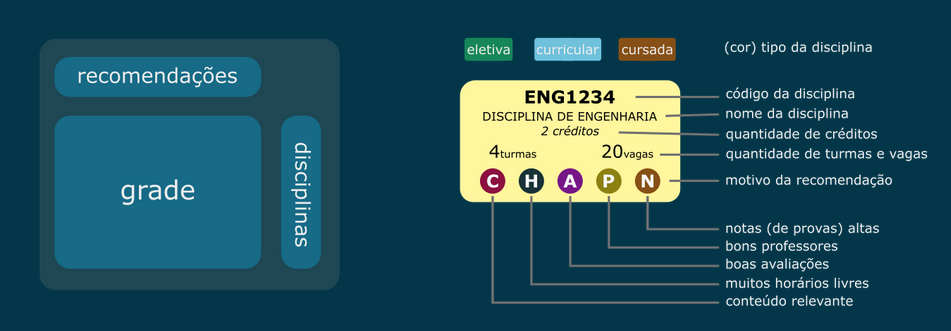
\includegraphics[width=360pt]{figuras/legenda-interface.png}
    \caption{Legenda da interface de criação de grade horária}
    \label{fig:legenda-interface}
    \end{center}
\end{figure}